\section{eo\-Proportional\-Op$<$ EOT $>$ Class Template Reference}
\label{classeo_proportional_op}\index{eoProportionalOp@{eoProportionalOp}}
The proportional versions: easy!  


{\tt \#include $<$eo\-Op\-Container.h$>$}

Inheritance diagram for eo\-Proportional\-Op$<$ EOT $>$::\begin{figure}[H]
\begin{center}
\leavevmode
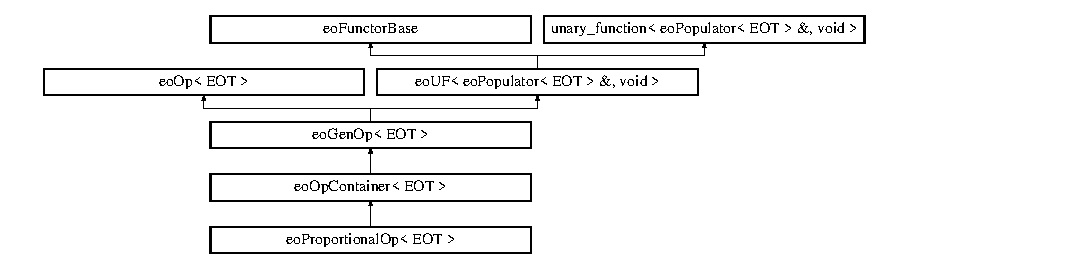
\includegraphics[height=3.18544cm]{classeo_proportional_op}
\end{center}
\end{figure}
\subsection*{Public Member Functions}
\begin{CompactItemize}
\item 
void {\bf apply} ({\bf eo\-Populator}$<$ {\bf EOT} $>$ \&\_\-pop)\label{classeo_proportional_op_a0}

\begin{CompactList}\small\item\em the function that will do the work \item\end{CompactList}\item 
virtual std::string {\bf class\-Name} () const \label{classeo_proportional_op_a1}

\end{CompactItemize}


\subsection{Detailed Description}
\subsubsection*{template$<$class EOT$>$ class eo\-Proportional\-Op$<$ EOT $>$}

The proportional versions: easy! 



Definition at line 135 of file eo\-Op\-Container.h.

The documentation for this class was generated from the following file:\begin{CompactItemize}
\item 
eo\-Op\-Container.h\end{CompactItemize}
